\section{ueaclib.c File Reference}
\label{ueaclib_8c}\index{ueaclib.c@{ueaclib.c}}
{\tt \#include $<$msp430x16x.h$>$}\par
{\tt \#include $<$signal.h$>$}\par
{\tt \#include $<$stdio.h$>$}\par
{\tt \#include \char`\"{}ueaclib.h\char`\"{}}\par
{\tt \#include \char`\"{}ueac.h\char`\"{}}\par
{\tt \#include \char`\"{}external\_\-flash.h\char`\"{}}\par
{\tt \#include \char`\"{}interpreter.h\char`\"{}}\par
{\tt \#include \char`\"{}filter.h\char`\"{}}\par
{\tt \#include \char`\"{}conversion.h\char`\"{}}\par
{\tt \#include \char`\"{}global.h\char`\"{}}\par
{\tt \#include \char`\"{}timer.h\char`\"{}}\par
{\tt \#include \char`\"{}calibrate.h\char`\"{}}\par


Include dependency graph for ueaclib.c:\begin{figure}[H]
\begin{center}
\leavevmode
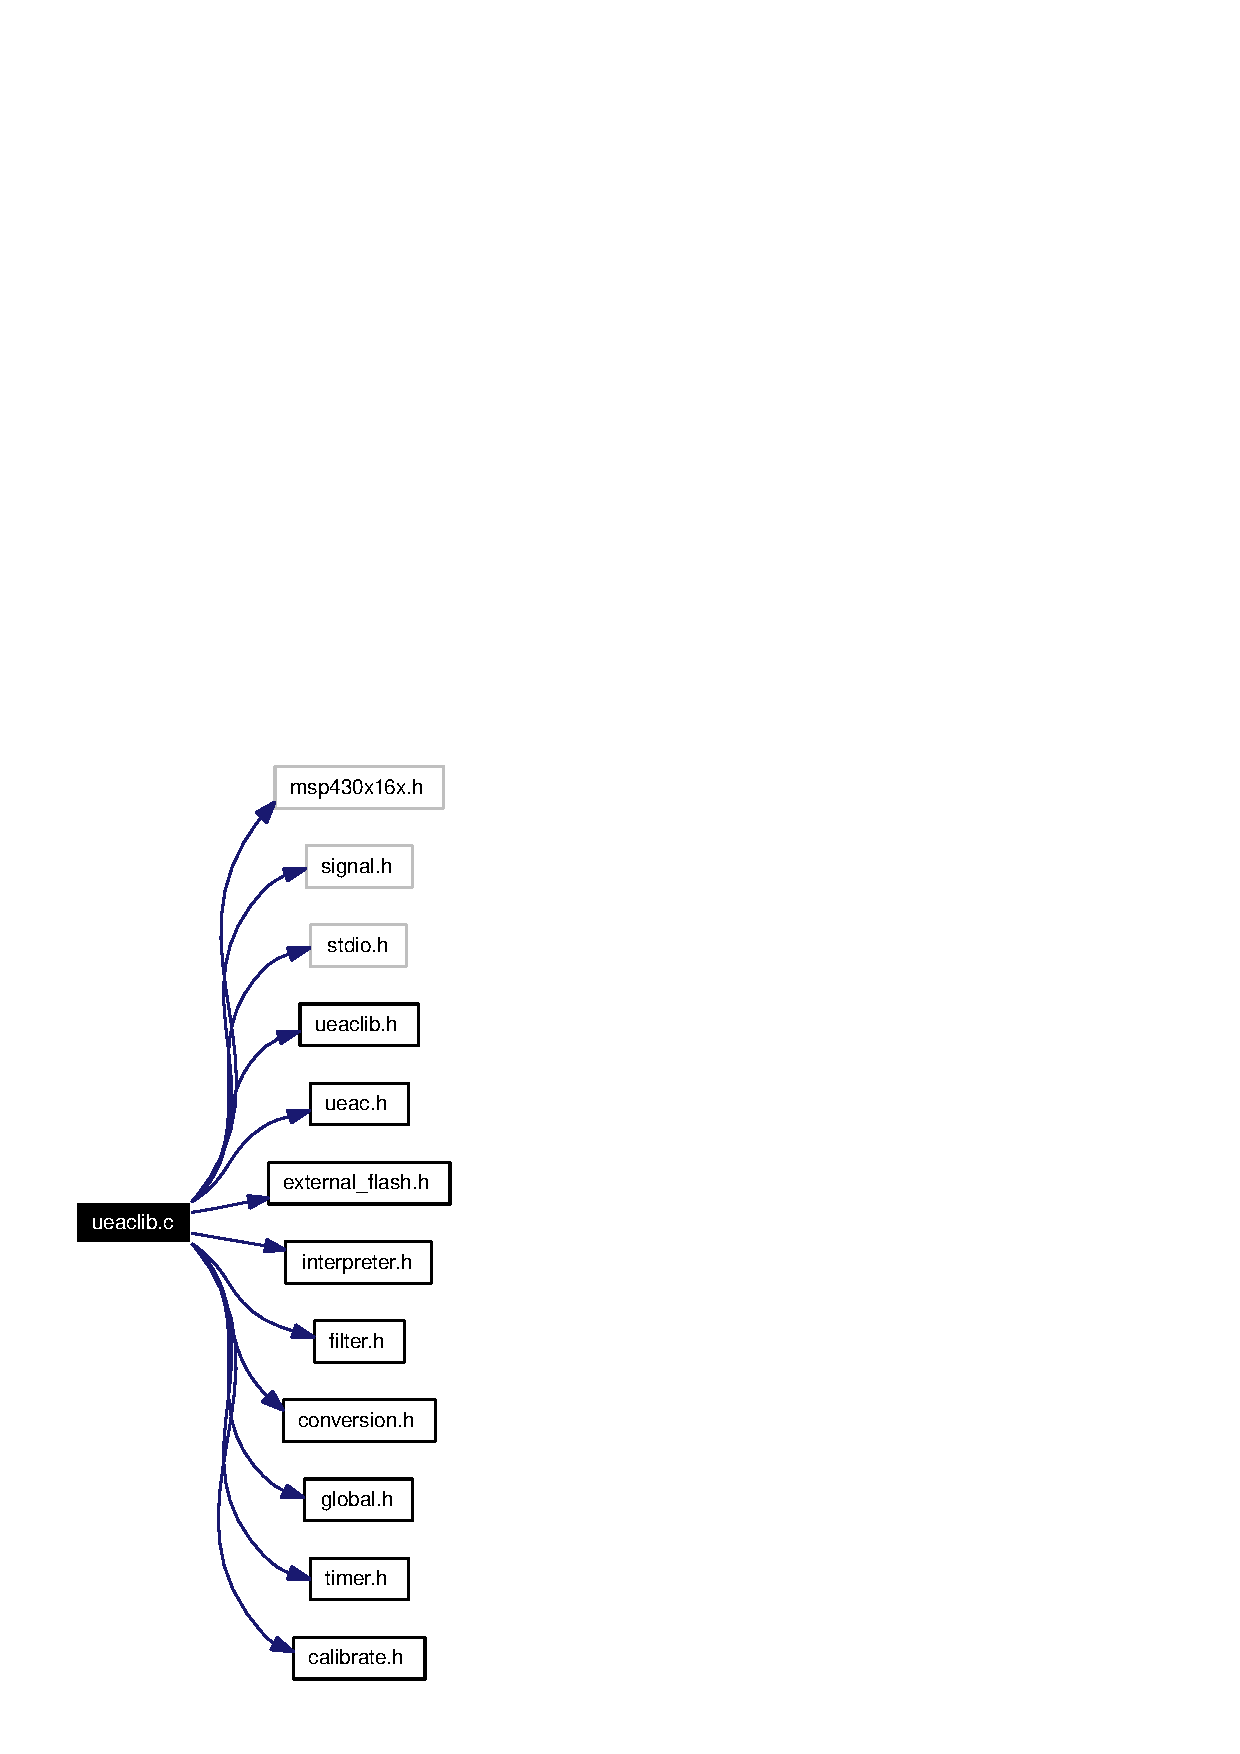
\includegraphics[width=108pt]{ueaclib_8c__incl}
\end{center}
\end{figure}
\subsection*{Defines}
\begin{CompactItemize}
\item 
\#define {\bf DELTA}~900
\item 
\#define {\bf PWM\_\-COUNT\_\-MASK}~0x1F
\end{CompactItemize}
\subsection*{Functions}
\begin{CompactItemize}
\item 
void {\bf init\_\-pins} (void)
\item 
void {\bf init\_\-spi\_\-0} (void)
\item 
void {\bf init\_\-serial\_\-1} (void)
\item 
void {\bf init\_\-timer\_\-a} (void)
\item 
void {\bf init\_\-dac} (void)
\item 
void {\bf init\_\-a2d} (void)
\item 
void {\bf start\_\-a2d\_\-converter} (void)
\item 
void {\bf Set\_\-DCO} (void)
\item 
void {\bf clear\_\-latches} (void)
\item 
void {\bf system\_\-reset} (void)
\item 
void {\bf init\_\-sys} (void)
\item 
unsigned char {\bf send\_\-spi\_\-byte} (unsigned char data\_\-byte)
\item 
int {\bf putchar} (int in\_\-char)
\item 
char {\bf getchar} (void)
\item 
void {\bf stop\_\-a2d\_\-converter} (void)
\item 
int {\bf wait\_\-a2d\_\-busy} (void)
\item 
void {\bf write\_\-analog\_\-mux} (unsigned char select)
\item 
void {\bf write\_\-current} (int {\bf channel}, int value\_\-u\-A)
\item 
void {\bf write\_\-dac} (int {\bf channel}, int value)
\item 
void {\bf led\_\-pwm} (int enable)
\item 
void {\bf clear\_\-led\_\-screen} (void)
\item 
void {\bf write\_\-led} (int {\bf channel}, int enable)
\item 
void {\bf write\_\-lla} (int {\bf channel}, int enable)
\end{CompactItemize}
\subsection*{Variables}
\begin{CompactItemize}
\item 
short {\bf dac\_\-translation} [$\,$]
\end{CompactItemize}


\subsection{Define Documentation}
\index{ueaclib.c@{ueaclib.c}!DELTA@{DELTA}}
\index{DELTA@{DELTA}!ueaclib.c@{ueaclib.c}}
\subsubsection{\setlength{\rightskip}{0pt plus 5cm}\#define DELTA~900}\label{ueaclib_8c_a0}




Definition at line 64 of file ueaclib.c.

Referenced by Set\_\-DCO().\index{ueaclib.c@{ueaclib.c}!PWM_COUNT_MASK@{PWM\_\-COUNT\_\-MASK}}
\index{PWM_COUNT_MASK@{PWM\_\-COUNT\_\-MASK}!ueaclib.c@{ueaclib.c}}
\subsubsection{\setlength{\rightskip}{0pt plus 5cm}\#define PWM\_\-COUNT\_\-MASK~0x1F}\label{ueaclib_8c_a1}




Definition at line 440 of file ueaclib.c.

Referenced by led\_\-pwm().

\subsection{Function Documentation}
\index{ueaclib.c@{ueaclib.c}!clear_latches@{clear\_\-latches}}
\index{clear_latches@{clear\_\-latches}!ueaclib.c@{ueaclib.c}}
\subsubsection{\setlength{\rightskip}{0pt plus 5cm}void clear\_\-latches (void)}\label{ueaclib_8c_a11}




Definition at line 101 of file ueaclib.c.

Referenced by init\_\-sys().

\footnotesize\begin{verbatim}101                          {
102   P1OUT=0x00;
103   P5OUT=0x3F;
104   P5OUT=0x00;
105 }
\end{verbatim}\normalsize 


\index{ueaclib.c@{ueaclib.c}!clear_led_screen@{clear\_\-led\_\-screen}}
\index{clear_led_screen@{clear\_\-led\_\-screen}!ueaclib.c@{ueaclib.c}}
\subsubsection{\setlength{\rightskip}{0pt plus 5cm}void clear\_\-led\_\-screen (void)}\label{ueaclib_8c_a23}




Definition at line 489 of file ueaclib.c.

Referenced by ueac\_\-execute\_\-instruction().

\footnotesize\begin{verbatim}489                              {
490   P1OUT=0;
491   P5OUT=0x07;
492   P5OUT=0;
493   P2OUT&=~0x01;
494 }
\end{verbatim}\normalsize 


\index{ueaclib.c@{ueaclib.c}!getchar@{getchar}}
\index{getchar@{getchar}!ueaclib.c@{ueaclib.c}}
\subsubsection{\setlength{\rightskip}{0pt plus 5cm}char getchar (void)}\label{ueaclib_8c_a16}




Definition at line 184 of file ueaclib.c.

Referenced by current\_\-output\_\-calibration(), and get\_\-command().

\footnotesize\begin{verbatim}184                    {
185   char rx_data;
186   while (!(IFG2&URXIFG1));
187   rx_data= RXBUF1;
188   return (rx_data);
189 }
\end{verbatim}\normalsize 


\index{ueaclib.c@{ueaclib.c}!init_a2d@{init\_\-a2d}}
\index{init_a2d@{init\_\-a2d}!ueaclib.c@{ueaclib.c}}
\subsubsection{\setlength{\rightskip}{0pt plus 5cm}void init\_\-a2d (void)}\label{ueaclib_8c_a8}


ADC12 Initialization Function \subsection{Overview}\label{ueaclib_8c_AA}
This project utilizes the first 5 channels of the A/D. Each of the channels is setup to use the 3.3V supply as the Reference. \par
\subsection{Converter Usage}\label{ueaclib_8c_BB}
\begin{TabularC}{3}
\hline
Pin&Function&Description \\\hline
P6.0&A/D 0&Reads External Mux for CH 0-7 \\\hline
P6.1&A/D 1&Reads External Mux for CH 8-15 \\\hline
P6.2&A/D 2&Reads External Mux for CH 16-23 \\\hline
P6.3&A/D 3&Reads CH24 \\\hline
P6.3&A/D 4&Reads VOP Voltage 10k//2.5k divider \\\hline
\end{TabularC}
\subsection{VOP Calculation}\label{ueaclib_8c_CC}
VOP\_\-Voltage = AD\_\-Counts\_\-VOP/248 \subsection{Converter Sampling Time Usage}\label{ueaclib_8c_D}
t\_\-sample$>$(Rs+2k)x9.011x40pf+800n\-S; Rs is the channel external input resistance - 200 ohms for u\-EAC\par
 t\_\-sample$>$2200x9.011x40pf+800n\-S=1.6u\-S 1.6u\-S = 12.8 clocks of the 8Mhz oscillator. Choose 16 for the sample clock divisor.\subsection{Converter Sampling Time Usage}\label{ueaclib_8c_D}


Definition at line 350 of file ueaclib.c.

Referenced by init\_\-sys().

\footnotesize\begin{verbatim}350                      {
351   // ADC12 Parameters
352   // Sample Hold Time - 16 clocks 
355   ADC12CTL0 = SHT1_2|SHT0_2|MSC|REF2_5V|REFON|ADC12ON; // sampling time set to 3.2uS 
356   ADC12CTL1 = SHP|CONSEQ0;                             // sample sequence of channels and then stop 
357   ADC12MCTL0 =  SREF_2|INCH_0;                         // Use Avcc (3.3V) as the reference, channels (0-7)   
358   ADC12MCTL1 =  SREF_2|INCH_1;                         // Use Avcc (3.3V) as the reference, channels (8-15)   
359   ADC12MCTL2 =  SREF_2|INCH_2;                         // Use Avcc (3.3V) as the reference, channels (16-23)   
360   ADC12MCTL3 =  EOS|SREF_2|INCH_3;                     // Use Avcc (3.3V) as the reference, channels (24)    
361 }
\end{verbatim}\normalsize 


\index{ueaclib.c@{ueaclib.c}!init_dac@{init\_\-dac}}
\index{init_dac@{init\_\-dac}!ueaclib.c@{ueaclib.c}}
\subsubsection{\setlength{\rightskip}{0pt plus 5cm}void init\_\-dac (void)}\label{ueaclib_8c_a7}




Definition at line 310 of file ueaclib.c.

Referenced by init\_\-sys().

\footnotesize\begin{verbatim}310                     {
311   // Dac 0 Controls Sources 
312   // Dac 1 Controls Sinks
313   // Parameters
314   // [14-13] DAC12SREFx (11) Use VeREF+->3.3V 
315   // [12] DAC12RES (0) 12-Bit Resolution  
316   // [11-10] DAC12LSELx (00) Load DAC on write to the DAC12_0DAT register
317   // [9] DAC12CALON (1) Calibration active, poll until this bit is clear 
318   // [8] DAC12IR (1) Input range = 1x
319   // [7-5] DAC12AMPx (111) High Speed, High Current 
320   // [4] DAC12DF (0) Straight Binary 
321   // [3] DAC12IE (0) Interrupt Disabled
322   // [2] DAC12IFG (x) Interrupt flag
323   // [1] DAC12ENC (1) Enable DAC conversion 
324   // [0] DAC12GRP (0) Channel grouping disabled 
325   DAC12_0CTL = DAC12SREF1|DAC12SREF0|DAC12CALON|DAC12IR|DAC12AMP2|DAC12AMP1|DAC12AMP0|DAC12ENC;
326   while (DAC12_0CTL&DAC12CALON);  // spin here until cal complete
327 }
\end{verbatim}\normalsize 


\index{ueaclib.c@{ueaclib.c}!init_pins@{init\_\-pins}}
\index{init_pins@{init\_\-pins}!ueaclib.c@{ueaclib.c}}
\subsubsection{\setlength{\rightskip}{0pt plus 5cm}void init\_\-pins (void)}\label{ueaclib_8c_a3}


{\em {\bf P1 Usage}\/} \begin{TabularC}{4}
\hline
Pin&Function&Direction&Select \\\hline
P1.0&Latch\_\-Data(0)&Output&Dio \\\hline
P1.1&Latch\_\-Data(1)&Output&Dio \\\hline
P1.2&Latch\_\-Data(2)&Output&Dio \\\hline
P1.3&Latch\_\-Data(3)&Output&Dio \\\hline
P1.4&Latch\_\-Data(4)&Output&Dio \\\hline
P1.5&Latch\_\-Data(5)&Output&Dio \\\hline
P1.6&Latch\_\-Data(6)&Output&Dio \\\hline
P1.7&Latch\_\-Data(7)&Output&Dio \\\hline
\end{TabularC}


{\em {\bf P2 Usage}\/} \begin{TabularC}{4}
\hline
Pin&Function&Direction&Select \\\hline
P2.0&LED\_\-OUT(24)&Output&Dio \\\hline
P2.1&LLA\_\-ENABLE(24)&Output&Dio \\\hline
P2.2&BSL(0) FTDI CHB TXD&Input&Dio \\\hline
P2.3&No Connect&Output&Dio \\\hline
P2.4&No Connect&Output&Dio \\\hline
P2.5&100k Pull-up Rosc&Input&Dio \\\hline
P2.6&No Connect&Output&Dio \\\hline
P2.7&FTDI n\-RTS&Input&Dio \\\hline
\end{TabularC}


{\em {\bf P3 Usage}\/} \begin{TabularC}{4}
\hline
Pin&Function&Direction&Select \\\hline
P3.0&FTDI n\-CTS&Output&Dio \\\hline
P3.1&SIMO-0&Output&{\bf Sel} \\\hline
P3.2&SOMI-0&Input&{\bf Sel} \\\hline
P3.3&SCK-0&Output&{\bf Sel} \\\hline
P3.4&UART0 TX&Output&{\bf Sel} \\\hline
P3.5&UART0 RX&Input&{\bf Sel} \\\hline
P3.6&UART1 TX&Output&{\bf Sel} \\\hline
P3.7&UART1 RX&Input&{\bf Sel} \\\hline
\end{TabularC}


{\em {\bf P4 Usage}\/} \begin{TabularC}{4}
\hline
Pin&Function&Direction&Select \\\hline
P4.0&SPI n\-CS DAC CH 0-7&Output&Dio \\\hline
P4.1&SPI n\-CS DAC CH 8-15&Output&Dio \\\hline
P4.2&SPI n\-CS DAC CH 16-23&Output&Dio \\\hline
P4.3&SPI n\-CS Serial Flash&Output&Dio \\\hline
P4.4&Analog Mux Select (0)&Output&Dio \\\hline
P4.5&Analog Mux Select (1)&Output&Dio \\\hline
P4.6&Analog Mux Select (2)&Output&Dio \\\hline
P4.7&8Mhz Osc Enable&Output&Dio \\\hline
\end{TabularC}


{\em {\bf P5 Usage}\/} \begin{TabularC}{4}
\hline
Pin&Function&Direction&Select \\\hline
P5.0&LED Latch Clk CH 0-7&Output&Dio \\\hline
P5.1&LED Latch Clk CH 8-15&Output&Dio \\\hline
P5.2&LED Latch Clk CH 16-23&Output&Dio \\\hline
P5.3&LLA Latch Clk CH 0-7&Output&Dio \\\hline
P5.4&LLA Latch Clk CH 8-15&Output&Dio \\\hline
P5.5&LLA Latch Clk CH 16-23&Output&Dio \\\hline
P5.6&No Connect&Output&Dio \\\hline
P5.7&No Connect&Output&Dio \\\hline
\end{TabularC}


{\em {\bf P6 Usage}\/} \begin{TabularC}{4}
\hline
Pin&Function&Direction&Select \\\hline
P6.0&VMUX\_\-OUT(0)&Input&{\bf Sel} \\\hline
P6.1&VMUX\_\-OUT(1)&Input&{\bf Sel} \\\hline
P6.2&VMUX\_\-OUT(2)&Input&{\bf Sel} \\\hline
P6.3&VMUX\_\-OUT(3)&Input&{\bf Sel} \\\hline
P6.4&VMUX\_\-OUT(4)&Input&{\bf Sel} \\\hline
P6.5&No Connect&Input&Dio \\\hline
P6.6&DAC Control CH24&Input (analog output)&{\bf Sel} \\\hline
P6.7&No Connect&Input&Dio \\\hline
\end{TabularC}


Definition at line 191 of file ueaclib.c.

Referenced by init\_\-sys().

\footnotesize\begin{verbatim}191                      {
206   P1SEL = 0x00;
207   P1OUT = 0x00;
208   P1DIR = 0xFF;
209 
224   P2SEL = 0x00;
225   P2OUT = 0x00;
226   P2DIR = 0x5B;
227 
242   P3SEL = 0xFE;
243   P3OUT = 0x00;
244   P3DIR = 0x5B;
245 
260   P4SEL = 0x00;
261   P4OUT = 0x8F;   
262   P4DIR = 0xFF; 
277   P5SEL = 0x00;
278   P5OUT = 0x00;
279   P5DIR = 0xFF; 
280 
295   P6SEL = 0x5F;
296   P6OUT = 0x00;
297   P6DIR = 0xA0; 
298 }
\end{verbatim}\normalsize 


\index{ueaclib.c@{ueaclib.c}!init_serial_1@{init\_\-serial\_\-1}}
\index{init_serial_1@{init\_\-serial\_\-1}!ueaclib.c@{ueaclib.c}}
\subsubsection{\setlength{\rightskip}{0pt plus 5cm}void init\_\-serial\_\-1 (void)}\label{ueaclib_8c_a5}




Definition at line 162 of file ueaclib.c.

Referenced by init\_\-sys().

\footnotesize\begin{verbatim}162                           {
163   char temp;
164   // Data Comm Port - Connected to FT2232 Port A
165   UCTL1 = CHAR + SWRST;
166   UTCTL1 = SSEL1 + SSEL0;
167 
168   // 19.2k init (3.686400 Mhz Clock)
169   UBR01=0xC0; 
170   UBR11=0x00;
171   UMCTL1=0x00; 
172   ME2 = 0x30;
173   UCTL1 = CHAR;
174   temp=RXBUF1;  // Flush the RX buffer 
175   temp=RXBUF1;  
176 }
\end{verbatim}\normalsize 


\index{ueaclib.c@{ueaclib.c}!init_spi_0@{init\_\-spi\_\-0}}
\index{init_spi_0@{init\_\-spi\_\-0}!ueaclib.c@{ueaclib.c}}
\subsubsection{\setlength{\rightskip}{0pt plus 5cm}void init\_\-spi\_\-0 (void)}\label{ueaclib_8c_a4}




Definition at line 140 of file ueaclib.c.

Referenced by init\_\-sys().

\footnotesize\begin{verbatim}140                        {
141   UCTL0 |= SWRST;                // Place USART into RESET 
142   UCTL0  = CHAR|SYNC|MM|SWRST;   // 8-bit,SPI,Master,Hold Module in RESET
143   UTCTL0 = CKPH|SSEL1|SSEL0|STC; // falling edge out,SMCLK,3-pin SPI (Works for LTC Parts)
144   // UTCTL0 = CKPL|SSEL1|SSEL0|STC; // falling edge out,SMCLK,3-pin SPI (Works for AT parts)
145   // LTC1660 DAC can handle a 5Mhz SCLK
146   // AT45DB041 Flash can handle 20Mhz SCLK 
147   UBR00  = 0x02;                 // Run at SMCLK/2 - 8Mhz/2=4Mhz for normal operation
148   UBR10  = 0x00;                 // Upper half of SCLK control 
149   ME1    = USPIE0;               // Enable the SPI module for UART0
150   UMCTL0 = 0x00;                 // Modulation control not used by SPI set to 0 according to User's Guide
151   UCTL0 &= ~SWRST;               // release USART from RESET 
152 }
\end{verbatim}\normalsize 


\index{ueaclib.c@{ueaclib.c}!init_sys@{init\_\-sys}}
\index{init_sys@{init\_\-sys}!ueaclib.c@{ueaclib.c}}
\subsubsection{\setlength{\rightskip}{0pt plus 5cm}void init\_\-sys (void)}\label{ueaclib_8c_a13}




Definition at line 79 of file ueaclib.c.

References clear\_\-latches(), init\_\-a2d(), init\_\-dac(), init\_\-pins(), init\_\-serial\_\-1(), init\_\-spi\_\-0(), init\_\-timer\_\-a(), and Set\_\-DCO().

Referenced by main().

\footnotesize\begin{verbatim}79                     {
80   unsigned int i;
81   WDTCTL = WDTPW + WDTHOLD;    // Stop watchdog
82   init_pins();                 // Setup the discrete I/O - important to enable 8Mhz crystal 
83   for (i = 0xFFFF;i>0;i--);    // Delay for XTAL and oscillator to fire up and settle
84   Set_DCO();                   // calibrate DCO using the 32.768Khz crystal to 3.686400 Mhz  
85   init_spi_0();
86   init_serial_1();             // initialize USB virtual serial port
87   init_timer_a();              
88   init_dac();
89   init_a2d();
90   clear_latches();
91   _EINT();                     // Global interrupt enable
92 }
\end{verbatim}\normalsize 




Here is the call graph for this function:\begin{figure}[H]
\begin{center}
\leavevmode
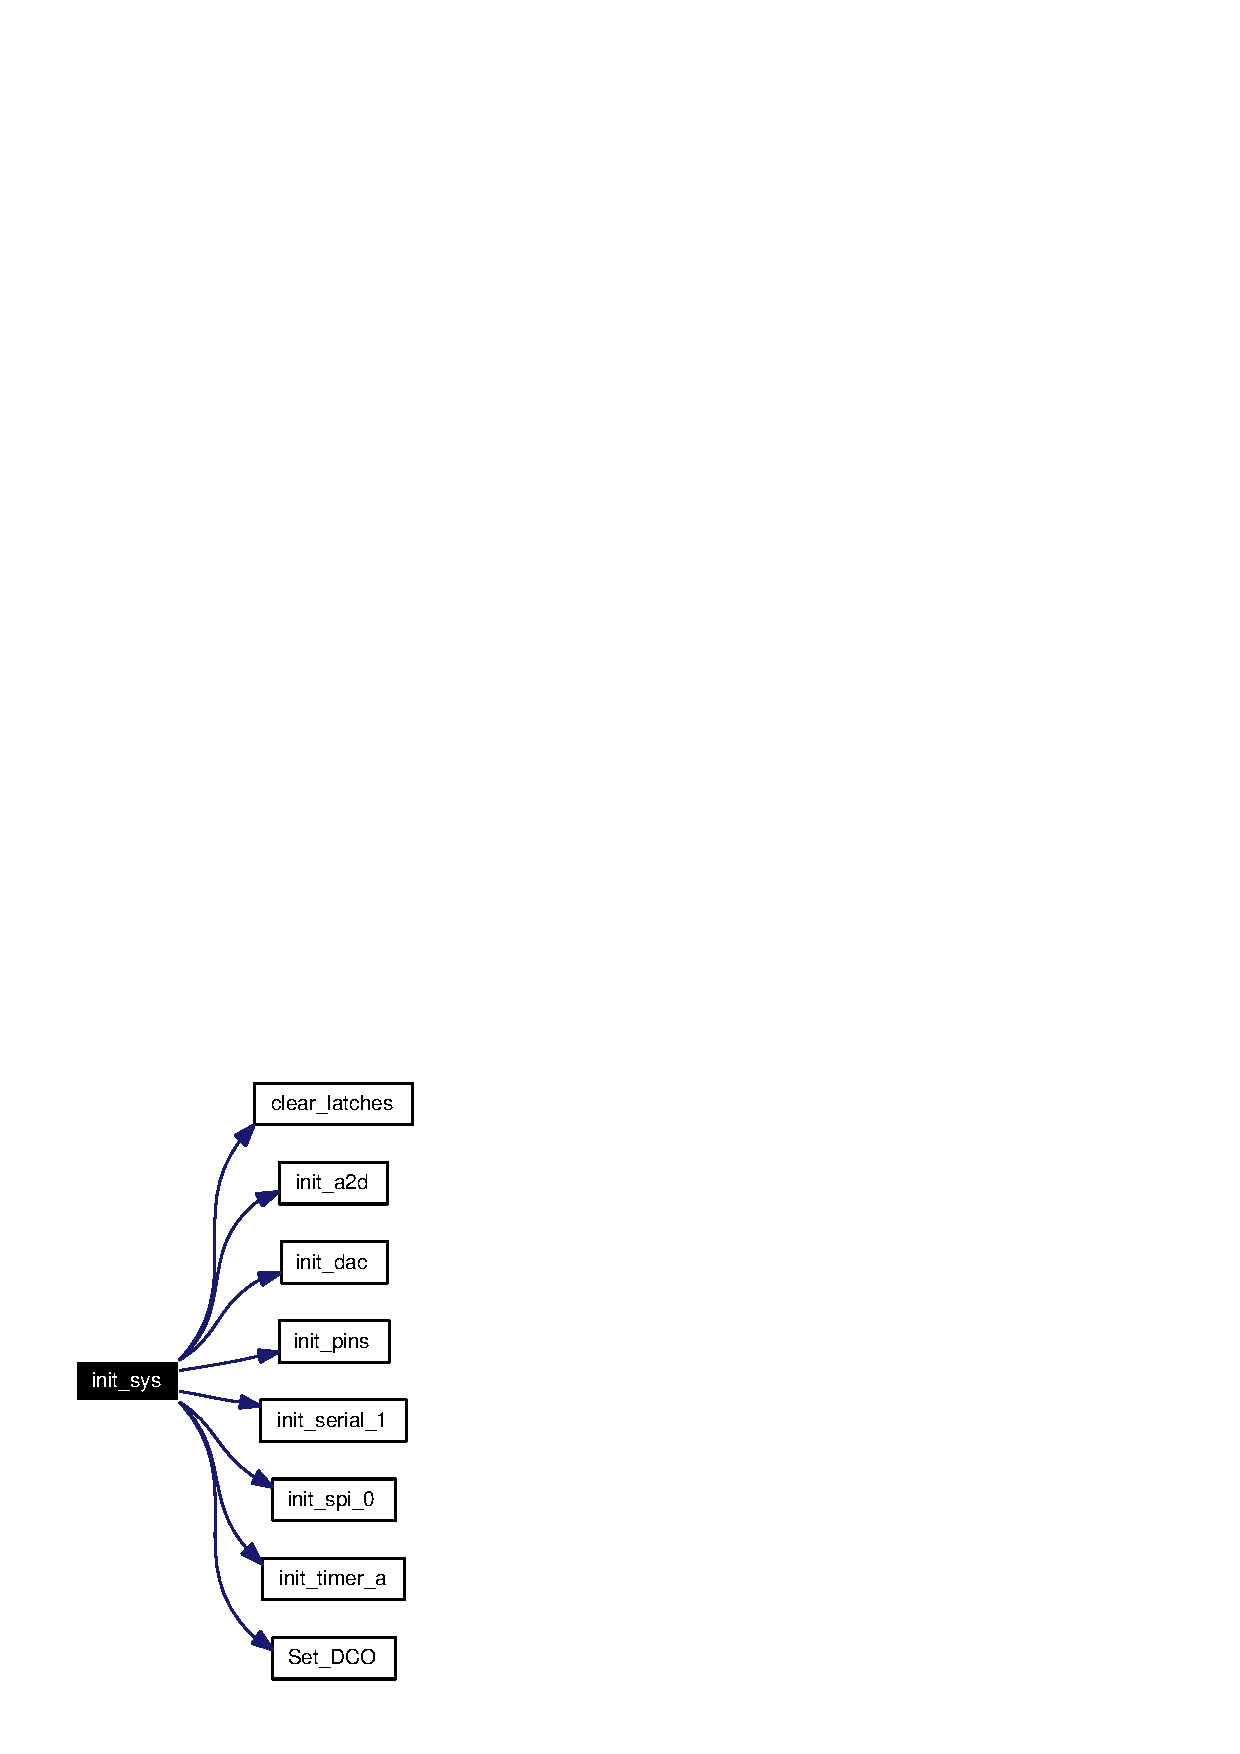
\includegraphics[width=99pt]{ueaclib_8c_a13_cgraph}
\end{center}
\end{figure}
\index{ueaclib.c@{ueaclib.c}!init_timer_a@{init\_\-timer\_\-a}}
\index{init_timer_a@{init\_\-timer\_\-a}!ueaclib.c@{ueaclib.c}}
\subsubsection{\setlength{\rightskip}{0pt plus 5cm}void init\_\-timer\_\-a (void)}\label{ueaclib_8c_a6}




Definition at line 300 of file ueaclib.c.

Referenced by init\_\-sys().

\footnotesize\begin{verbatim}300                         {
301   // SMCLK SOURCE (3.686400Mhz)
302   // Timer in Continuous Mode 
303   // Clear the timer register (TAR)
304   // Compare 1 used as main time base at 1.25mS. 
305   TACTL=TASSEL1|MC1|TACLR;  // Timer a sourced from 3.686400 Mhz SMCLK, continuous mode
306   TACCR0=0x900;             // 100uS interrupt rate
307   TACCTL0=CCIE;             // Enable the timer interrupt
308 }
\end{verbatim}\normalsize 


\index{ueaclib.c@{ueaclib.c}!led_pwm@{led\_\-pwm}}
\index{led_pwm@{led\_\-pwm}!ueaclib.c@{ueaclib.c}}
\subsubsection{\setlength{\rightskip}{0pt plus 5cm}void led\_\-pwm (int {\em enable})}\label{ueaclib_8c_a22}




Definition at line 441 of file ueaclib.c.

References high\_\-time\_\-limit, and PWM\_\-COUNT\_\-MASK.

Referenced by timer\_\-a0\_\-irq().

\footnotesize\begin{verbatim}441                           {
442   static unsigned char counter=0;
443   if (enable) {
444     counter++;
445     counter&=PWM_COUNT_MASK; 
446     if (!counter) {
447       P1OUT=0xFF;
448       P5OUT=0x07;
449       P5OUT=0;
450       P2OUT|=0x01;
451     }
452     P1OUT=0xFF;
453     if (counter>=high_time_limit[0]) P1OUT&=~0x01;
454     if (counter>=high_time_limit[1]) P1OUT&=~0x02;
455     if (counter>=high_time_limit[2]) P1OUT&=~0x04;
456     if (counter>=high_time_limit[3]) P1OUT&=~0x08;
457     if (counter>=high_time_limit[4]) P1OUT&=~0x10;
458     if (counter>=high_time_limit[5]) P1OUT&=~0x20;
459     if (counter>=high_time_limit[6]) P1OUT&=~0x40;
460     if (counter>=high_time_limit[7]) P1OUT&=~0x80;
461     P5OUT=0x01;
462     P5OUT=0x00;
463     P1OUT=0xFF;
464     if (counter>=high_time_limit[8]) P1OUT&=~0x01;
465     if (counter>=high_time_limit[9]) P1OUT&=~0x02;
466     if (counter>=high_time_limit[10]) P1OUT&=~0x04;
467     if (counter>=high_time_limit[11]) P1OUT&=~0x08;
468     if (counter>=high_time_limit[12]) P1OUT&=~0x10;
469     if (counter>=high_time_limit[13]) P1OUT&=~0x20;
470     if (counter>=high_time_limit[14]) P1OUT&=~0x40;
471     if (counter>=high_time_limit[15]) P1OUT&=~0x80;
472     P5OUT=0x02;
473     P5OUT=0x00;
474     P1OUT=0xFF;
475     if (counter>=high_time_limit[16]) P1OUT&=~0x01;
476     if (counter>=high_time_limit[17]) P1OUT&=~0x02;
477     if (counter>=high_time_limit[18]) P1OUT&=~0x04;
478     if (counter>=high_time_limit[19]) P1OUT&=~0x08;
479     if (counter>=high_time_limit[20]) P1OUT&=~0x10;
480     if (counter>=high_time_limit[21]) P1OUT&=~0x20;
481     if (counter>=high_time_limit[22]) P1OUT&=~0x40;
482     if (counter>=high_time_limit[23]) P1OUT&=~0x80;
483     P5OUT=0x04;
484     P5OUT=0x00;
485     if (counter>=high_time_limit[24]) P2OUT&=~0x01;
486   }
487 }
\end{verbatim}\normalsize 


\index{ueaclib.c@{ueaclib.c}!putchar@{putchar}}
\index{putchar@{putchar}!ueaclib.c@{ueaclib.c}}
\subsubsection{\setlength{\rightskip}{0pt plus 5cm}int putchar (int {\em in\_\-char})}\label{ueaclib_8c_a15}




Definition at line 178 of file ueaclib.c.

\footnotesize\begin{verbatim}178                         {
179   while (!(IFG2&UTXIFG1));
180   TXBUF1=in_char;
181   return(0);
182 }
\end{verbatim}\normalsize 


\index{ueaclib.c@{ueaclib.c}!send_spi_byte@{send\_\-spi\_\-byte}}
\index{send_spi_byte@{send\_\-spi\_\-byte}!ueaclib.c@{ueaclib.c}}
\subsubsection{\setlength{\rightskip}{0pt plus 5cm}unsigned char send\_\-spi\_\-byte (unsigned char {\em data\_\-byte})}\label{ueaclib_8c_a14}




Definition at line 154 of file ueaclib.c.

\footnotesize\begin{verbatim}154                                                      {
155   TXBUF0 = data_byte;        // buffer 1 write  
156   while(!(UTCTL0&0x01));     // wait until transmitter empty
157   return(RXBUF0);            // return any received data
158                              // No data returned from DAC
159                              // SPI flash returns read data
160 }
\end{verbatim}\normalsize 


\index{ueaclib.c@{ueaclib.c}!Set_DCO@{Set\_\-DCO}}
\index{Set_DCO@{Set\_\-DCO}!ueaclib.c@{ueaclib.c}}
\subsubsection{\setlength{\rightskip}{0pt plus 5cm}void Set\_\-DCO (void)}\label{ueaclib_8c_a10}




Definition at line 107 of file ueaclib.c.

References DELTA.

Referenced by init\_\-sys().

\footnotesize\begin{verbatim}107                     { 
108   unsigned int Compare, Oldcapture = 0;
109   CCTL0 = 0x0000;                       // this too - see next comment
110   CCTL1 = 0x0000;                       // see if this fixes the clock cal issue
111   CCTL2 = 0x0000;
112   CCTL2 = CCIS0 + CM0 + CAP;            // Define CCR2, CAP, ACLK
113   TACTL = TASSEL1 + TACLR + MC1;        // SMCLK, continous mode
114   while (1) {
115     while ((CCTL2 & CCIFG) != CCIFG);   // Wait until capture occured!
116     CCTL2 &= ~CCIFG;                    // Capture occured, clear flag
117     Compare = CCR2;                     // Get current captured SMCLK
118     Compare = Compare - Oldcapture;     // SMCLK difference
119     Oldcapture = CCR2;                  // Save current captured SMCLK
120     if (DELTA == Compare) {
121       break;                            // if equal, leave "while(1)"
122     }
123     else if (DELTA < Compare) {         // DCO is too fast, slow it down
124       DCOCTL--;
125       if (DCOCTL == 0xFF) {             // Did DCO roll under?
126         BCSCTL1--;                      // Select next lower RSEL
127       }
128     }
129     else {                      
130       DCOCTL++;
131       if (DCOCTL == 0x00) {             // Did DCO roll over?
132         BCSCTL1++;                      // Select next higher RSEL
133       }
134     }
135   }  
136   CCTL2 = 0;                              // Stop CCR2 function
137   TACTL = 0;                              // Stop Timer_A
138 }
\end{verbatim}\normalsize 


\index{ueaclib.c@{ueaclib.c}!start_a2d_converter@{start\_\-a2d\_\-converter}}
\index{start_a2d_converter@{start\_\-a2d\_\-converter}!ueaclib.c@{ueaclib.c}}
\subsubsection{\setlength{\rightskip}{0pt plus 5cm}void start\_\-a2d\_\-converter (void)}\label{ueaclib_8c_a9}




Definition at line 363 of file ueaclib.c.

Referenced by timer\_\-a0\_\-irq().

\footnotesize\begin{verbatim}363                                {
364   ADC12CTL0|=ENC|ADC12SC;                    // start the converter 
365 }  
\end{verbatim}\normalsize 


\index{ueaclib.c@{ueaclib.c}!stop_a2d_converter@{stop\_\-a2d\_\-converter}}
\index{stop_a2d_converter@{stop\_\-a2d\_\-converter}!ueaclib.c@{ueaclib.c}}
\subsubsection{\setlength{\rightskip}{0pt plus 5cm}void stop\_\-a2d\_\-converter (void)}\label{ueaclib_8c_a17}




Definition at line 367 of file ueaclib.c.

\footnotesize\begin{verbatim}367                               {
368   ADC12CTL0&=~ENC;                           // stop the converter 
369 }  
\end{verbatim}\normalsize 


\index{ueaclib.c@{ueaclib.c}!system_reset@{system\_\-reset}}
\index{system_reset@{system\_\-reset}!ueaclib.c@{ueaclib.c}}
\subsubsection{\setlength{\rightskip}{0pt plus 5cm}void system\_\-reset (void)}\label{ueaclib_8c_a12}




Definition at line 94 of file ueaclib.c.

Referenced by ueac\_\-execute\_\-instruction().

\footnotesize\begin{verbatim}94                         {
95   _DINT();
96   WDTCTL = WDTPW|WDTCNTCL|WDTIS_3;  // start the watchdog, SMCLK ticks until reset 
97   P4OUT=0x8F;
98   while (1);                        // wedge here until the dog resets the core
99 }
\end{verbatim}\normalsize 


\index{ueaclib.c@{ueaclib.c}!wait_a2d_busy@{wait\_\-a2d\_\-busy}}
\index{wait_a2d_busy@{wait\_\-a2d\_\-busy}!ueaclib.c@{ueaclib.c}}
\subsubsection{\setlength{\rightskip}{0pt plus 5cm}int wait\_\-a2d\_\-busy (void)}\label{ueaclib_8c_a18}




Definition at line 371 of file ueaclib.c.

\footnotesize\begin{verbatim}371                         {
372   int count=0;
373   while (ADC12CTL1&ADC12BUSY) count++;
374   return count;
375 }
\end{verbatim}\normalsize 


\index{ueaclib.c@{ueaclib.c}!write_analog_mux@{write\_\-analog\_\-mux}}
\index{write_analog_mux@{write\_\-analog\_\-mux}!ueaclib.c@{ueaclib.c}}
\subsubsection{\setlength{\rightskip}{0pt plus 5cm}void write\_\-analog\_\-mux (unsigned char {\em select})}\label{ueaclib_8c_a19}




Definition at line 377 of file ueaclib.c.

Referenced by timer\_\-a0\_\-irq().

\footnotesize\begin{verbatim}377                                             {
378   select&=0x07;   // clamp the input to 7 
379   select<<=4;     // shift to align with bits 6-4 (mux select bits)
380   P4OUT&=0x8F;    // clear the mux select bits
381   P4OUT|=select;  // "or" in the new select value
382 }
\end{verbatim}\normalsize 


\index{ueaclib.c@{ueaclib.c}!write_current@{write\_\-current}}
\index{write_current@{write\_\-current}!ueaclib.c@{ueaclib.c}}
\subsubsection{\setlength{\rightskip}{0pt plus 5cm}void write\_\-current (int {\em channel}, int {\em value\_\-u\-A})}\label{ueaclib_8c_a20}




Definition at line 384 of file ueaclib.c.

References dac\_\-translation, cal::i\_\-200u\-A\_\-offset, cal::i\_\-zero\_\-offset, ueac::pin\_\-cal, ueac\_\-state, and write\_\-dac().

Referenced by current\_\-output\_\-calibration(), evaluate\_\-lla(), lla\_\-disable(), lla\_\-enable(), main(), print\_\-grid\_\-i(), scan\_\-probes(), and ueac\_\-execute\_\-instruction().

\footnotesize\begin{verbatim}384                                              {
385   if (value_uA>200) value_uA=200;
386   if (value_uA<-200) value_uA=-200;
387   if (value_uA==0) {
388     write_dac(channel,(dac_translation[200]+ueac_state.pin_cal[channel].i_zero_offset));
389   }
390   else {
391     write_dac(channel,dac_translation[200-value_uA]+ueac_state.pin_cal[channel].i_200uA_offset);
392   }
393 }
\end{verbatim}\normalsize 




Here is the call graph for this function:\begin{figure}[H]
\begin{center}
\leavevmode
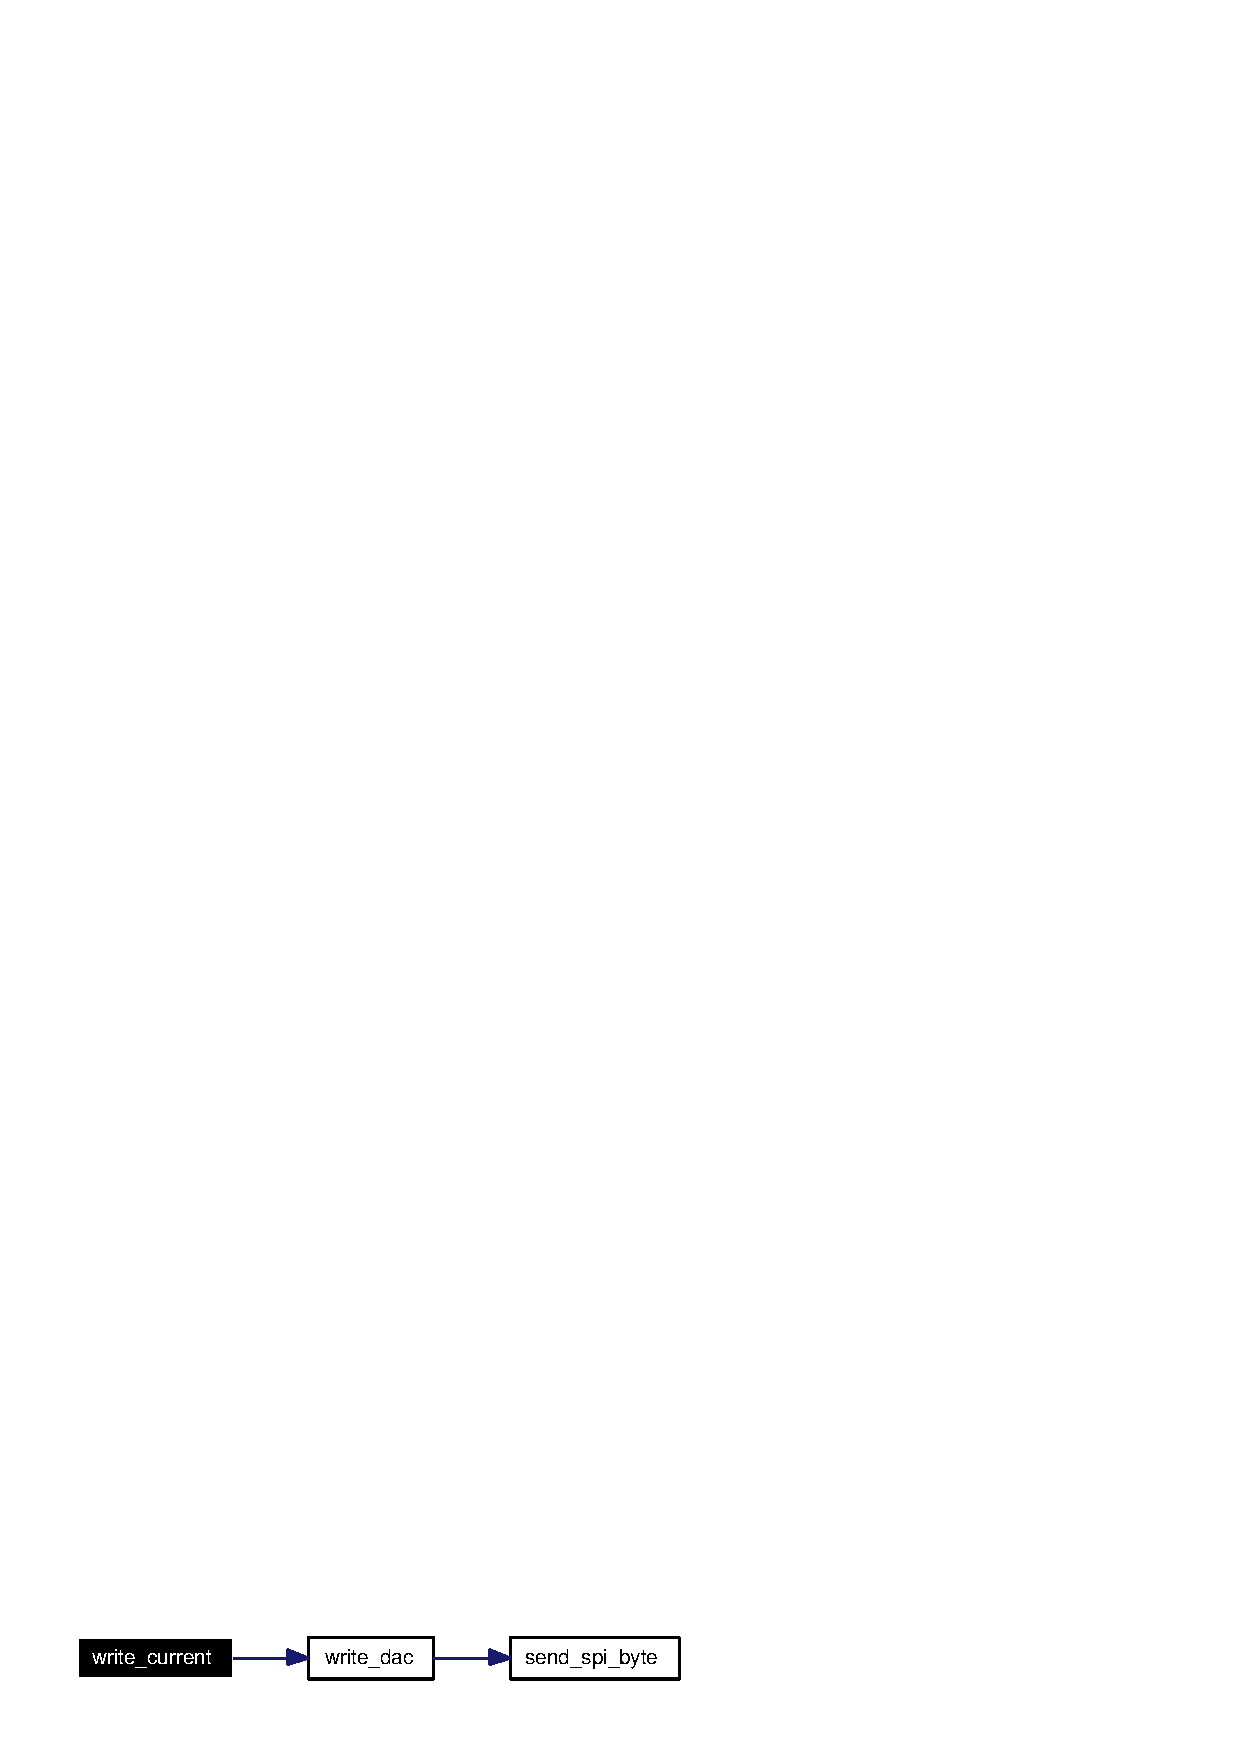
\includegraphics[width=163pt]{ueaclib_8c_a20_cgraph}
\end{center}
\end{figure}
\index{ueaclib.c@{ueaclib.c}!write_dac@{write\_\-dac}}
\index{write_dac@{write\_\-dac}!ueaclib.c@{ueaclib.c}}
\subsubsection{\setlength{\rightskip}{0pt plus 5cm}void write\_\-dac (int {\em channel}, int {\em value})}\label{ueaclib_8c_a21}




Definition at line 395 of file ueaclib.c.

References send\_\-spi\_\-byte().

Referenced by current\_\-output\_\-calibration(), and write\_\-current().

\footnotesize\begin{verbatim}395                                       {
396   // write_dac(channel,value)
397   // channel = 0-24 where the channels are the control voltages for the current sources. The current 
398   // sources are labeled starting at the top left corner as follows.
399   //  0  1  2  3  4
400   //  5  6  7  8  9
401   // 10 11 12 13 14
402   // 15 16 17 18 19
403   // 20 21 22 23 24
404   //
405   // Value = 0-1023 (10-bit) where the number represents a control voltage that is 0-3.3v. Each bit represents 
406   // a voltage of 3.3v/1023 or 3.22mV. 
407   //
408   // Hardware Note: Channels 0-23 are implemented by external SPI octal dacs (Linear LTC1660 components). Channel 
409   // 24 is implemented using DAC0 on the MSP430 
410   // 
411   // Initial Version BH 11/1/05
412 
413   if (channel < 8) {
414     P4OUT&=~0x01;                                   // assert the proper chip select
415     channel++;                                      // increment the channel number LTC1660 channels run from 1-8   
416   }           
417   else if (channel < 16) {
418     P4OUT&=~0x02;                                   // assert the proper chip select
419     channel-=7;                                     // bring channel number into range 1-8
420   } 
421   else if (channel < 24) {
422     P4OUT&=~0x04;                                   // assert the proper chip select
423     channel-=15;                                    // bring channel number into range 1-8
424   }
425   else if (channel == 24) {
426     DAC12_0DAT=value<<2;                            // Shift up to a 12-bit number and write to the MSP430 DAC0 
427     return;                                         // This is all to do for the MSP430 DAC case, exit...
428   }
429   else {                                            // channel number provided is too large, exit... 
430     return;
431   }
432   value=(value&0x03FF)<<2;                          // mask and shift the value to align properly in the dac sentence
433   channel<<=4;
434   *(((unsigned char *) &value)+1)|=((unsigned char) channel); // "or" in the channel number to the value data
435   send_spi_byte(*(((unsigned char *) &value)+1));             // send the high byte 
436   send_spi_byte(*((unsigned char *) &value));                 // send the high byte 
437   P4OUT|=0x0F;                                                // deassert all of the spi dac chip selects   
438 }
\end{verbatim}\normalsize 




Here is the call graph for this function:\begin{figure}[H]
\begin{center}
\leavevmode
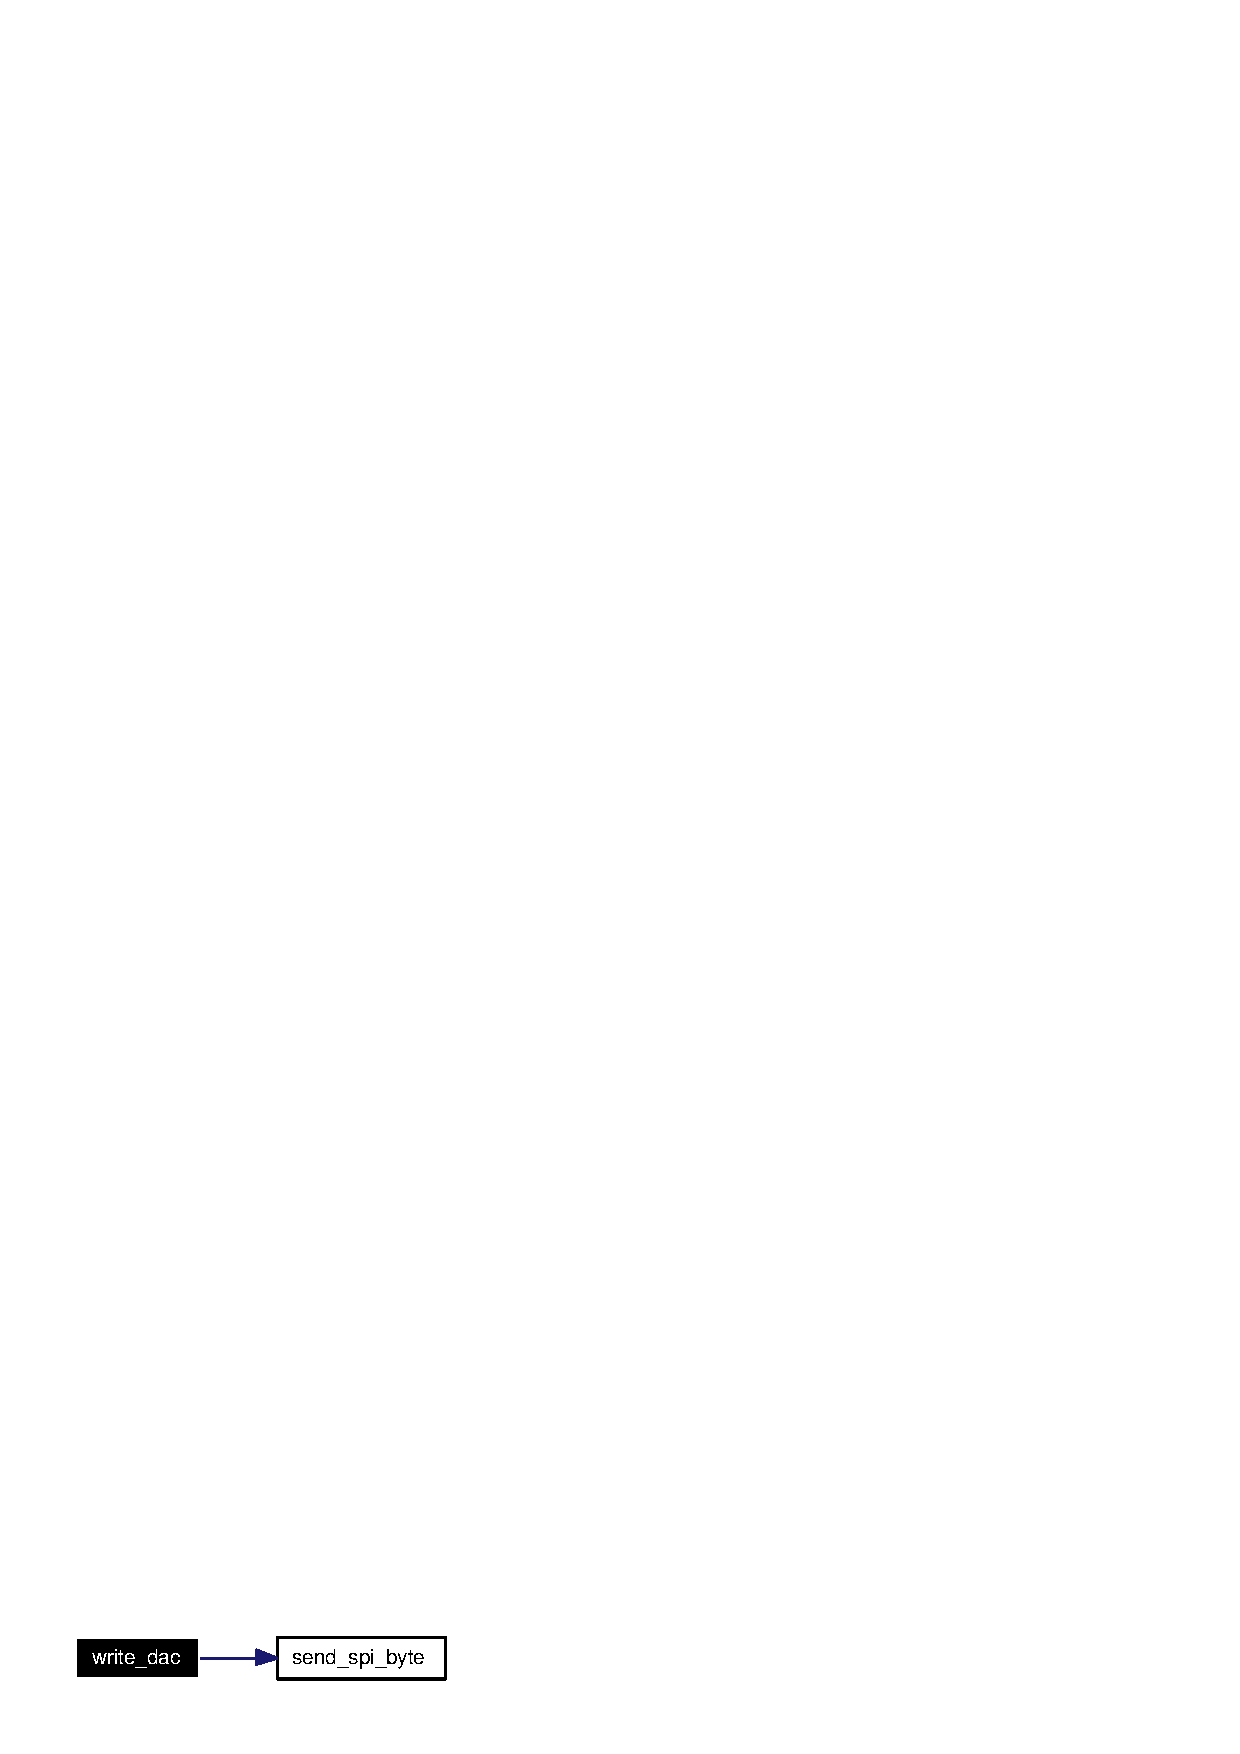
\includegraphics[width=107pt]{ueaclib_8c_a21_cgraph}
\end{center}
\end{figure}
\index{ueaclib.c@{ueaclib.c}!write_led@{write\_\-led}}
\index{write_led@{write\_\-led}!ueaclib.c@{ueaclib.c}}
\subsubsection{\setlength{\rightskip}{0pt plus 5cm}void write\_\-led (int {\em channel}, int {\em enable})}\label{ueaclib_8c_a24}




Definition at line 497 of file ueaclib.c.

Referenced by current\_\-output\_\-calibration(), main(), and scan\_\-leds().

\footnotesize\begin{verbatim}497                                          {
498   static unsigned long led_state = 0x00000000;
499   if (enable) {
500     if (channel<8) {
501       *((unsigned char *) &led_state) |= 0x01<<channel;       // Save the new state of the LED in led_state
502       P1OUT=*((unsigned char *) &led_state);                  // Place the relevant byte of led_state on the latch bus 
503       P5OUT|=0x01;                                            // strobe the chip select for the target latch
504       P5OUT&=~0x01;                                           // clear the chip select bit
505     }
506     else if (channel<16) {
507       channel-=8;
508       *(((unsigned char *) &led_state)+1) |= 0x01<<channel;  
509       P1OUT=*(((unsigned char *) &led_state)+1);  
510       P5OUT=0x02;
511       P5OUT&=~0x02;                                           // clear the chip select bit
512     }
513     else if (channel<24) {
514       channel-=16;
515       *(((unsigned char *) &led_state)+2) |= 0x01<<channel;  
516       P1OUT=*(((unsigned char *) &led_state)+2);  
517       P5OUT=0x04;
518       P5OUT&=~0x04;                                           // clear the chip select bit
519     }
520     else if (channel==24) {
521       *(((unsigned char *) &led_state)+3) |= 0x01;  
522       P2OUT|=0x01;
523     }
524   }
525   else {
526     if (channel<8) {
527       *((unsigned char *) &led_state) &= ~(0x01<<channel);  
528       P1OUT=*((unsigned char *) &led_state);  
529       P5OUT=0x01;
530       P5OUT&=~0x01;                                           // clear the chip select bit
531     }
532     else if (channel<16) {
533       channel-=8;
534       *(((unsigned char *) &led_state)+1) &= ~(0x01<<channel);  
535       P1OUT=*(((unsigned char *) &led_state)+1);  
536       P5OUT=0x02;
537       P5OUT&=~0x02;                                           // clear the chip select bit
538     }
539     else if (channel<24) {
540       channel-=16;
541       *(((unsigned char *) &led_state)+2) &= ~(0x01<<channel);  
542       P1OUT=*(((unsigned char *) &led_state)+2);  
543       P5OUT=0x04;
544       P5OUT&=~0x04;                                           // clear the chip select bit
545     }
546     else if (channel==24) {
547       *(((unsigned char *) &led_state)+3) &= 0xFE;  
548       P2OUT&=0xFE;
549     }
550   }
551 }
\end{verbatim}\normalsize 


\index{ueaclib.c@{ueaclib.c}!write_lla@{write\_\-lla}}
\index{write_lla@{write\_\-lla}!ueaclib.c@{ueaclib.c}}
\subsubsection{\setlength{\rightskip}{0pt plus 5cm}void write\_\-lla (int {\em channel}, int {\em enable})}\label{ueaclib_8c_a25}




Definition at line 553 of file ueaclib.c.

Referenced by current\_\-output\_\-calibration(), lla\_\-add(), lla\_\-disable(), lla\_\-enable(), main(), print\_\-grid\_\-i(), and scan\_\-probes().

\footnotesize\begin{verbatim}553                                          {
554   static unsigned long lla_state = 0x00000000;
555   if (enable) {
556     if (channel<8) {
557       *((unsigned char *) &lla_state) |= 0x01<<channel;       // Save the new state of the LED in lla_state
558       P1OUT=*((unsigned char *) &lla_state);                  // Place the relevant byte of lla_state on the latch bus 
559       P5OUT|=0x08;                                            // strobe the chip select for the target latch
560       P5OUT&=~0x08;                                           // clear the chip select bit
561     }
562     else if (channel<16) {
563       channel-=8;
564       *(((unsigned char *) &lla_state)+1) |= 0x01<<channel;  
565       P1OUT=*(((unsigned char *) &lla_state)+1);  
566       P5OUT=0x10;
567       P5OUT&=~0x10;                                           // clear the chip select bit
568     }
569     else if (channel<24) {
570       channel-=16;
571       *(((unsigned char *) &lla_state)+2) |= 0x01<<channel;  
572       P1OUT=*(((unsigned char *) &lla_state)+2);  
573       P5OUT=0x20;
574       P5OUT&=~0x20;                                           // clear the chip select bit
575     }
576     else if (channel==24) {
577       *(((unsigned char *) &lla_state)+3) |= 0x01;  
578       P2OUT|=0x02;
579     }
580   }
581   else {
582     if (channel<8) {
583       *((unsigned char *) &lla_state) &= ~(0x01<<channel);  
584       P1OUT=*((unsigned char *) &lla_state);  
585       P5OUT=0x08;
586       P5OUT&=~0x08;                                           // clear the chip select bit
587     }
588     else if (channel<16) {
589       channel-=8;
590       *(((unsigned char *) &lla_state)+1) &= ~(0x01<<channel);  
591       P1OUT=*(((unsigned char *) &lla_state)+1);  
592       P5OUT=0x10;
593       P5OUT&=~0x10;                                           // clear the chip select bit
594     }
595     else if (channel<24) {
596       channel-=16;
597       *(((unsigned char *) &lla_state)+2) &= ~(0x01<<channel);  
598       P1OUT=*(((unsigned char *) &lla_state)+2);  
599       P5OUT=0x20;
600       P5OUT&=~0x20;                                           // clear the chip select bit
601     }
602     else if (channel==24) {
603       *(((unsigned char *) &lla_state)+3) &= 0xFE;  
604       P2OUT&=0xFD;
605     }
606   }
607 }
\end{verbatim}\normalsize 




\subsection{Variable Documentation}
\index{ueaclib.c@{ueaclib.c}!dac_translation@{dac\_\-translation}}
\index{dac_translation@{dac\_\-translation}!ueaclib.c@{ueaclib.c}}
\subsubsection{\setlength{\rightskip}{0pt plus 5cm}short {\bf dac\_\-translation}[$\,$]}\label{ueaclib_8c_a2}




Definition at line 45 of file cal\_\-table.h.

Referenced by current\_\-output\_\-calibration(), and write\_\-current().